% Description: This is a recommended Latex template of the Department of Mathematics and Social Science
% SIBAU for BSM final year project, which can only be used for academic purposes. 
% BSM final year project report will be only submitted and accepted in this template. 
% Note: BSM project report/dissertation/thesis writing in other template be accepted by the
% department of Mathematics and Social Science, department of computer science, SIBAU.
% Author: H.A.M.S., Syed, K.Ali
% Created on: 01 December 2019
% Update on: 20 January 2020
% Update on: 25 October 2023
% Updated on: 03 September 2025
% Contact: syed.hyderali@iba-suk.edu.pk, khurshed.ali@iba-suk.edu.pk
% @copyright 2019: This template is strictly not allowed to be published anywhere on the public domains
% without the permission of the author.

% MAIN DOCUMENT CLASS - Use 'print' option for final printed version (removes colors for b/w printing)
\documentclass[print]{dissertation} % for printing the final version of Thesis
%\documentclass[]{dissertation} % Use this line instead for digital/colored version
%\color{sibau-dark-blue} % Uncomment to set a specific color scheme if needed
\usepackage{booktabs}
\usepackage{adjustbox}
\usepackage{pgfplots}
\pgfplotsset{compat=1.18}
\usetikzlibrary{arrows.meta,positioning,shapes.geometric,calc,fit,backgrounds}


% PACKAGES - Essential packages for document formatting
\usepackage[english]{babel} % Language support
\usepackage{csquotes} % Improved quotation handling
\usepackage[backend=biber, style=numeric]{biblatex} % Bibliography management with biber backend
\addbibresource{dissertation.bib} % Path to your bibliography file
%\usepackage{hyperref} % Creates clickable links in PDF

% CAPTION FORMATTING - Centers all figure and table captions
\captionsetup{justification=centering} % Remove this line if you prefer left-justified captions

%%%%%%%%%%%%%%%%%%%%%% begin document %%%%%%%%%%%%%%%%%%%%%%%%%
\begin{document}

% THESIS METADATA - Fill in your specific information here
\title[Hands On Approach]{CRYPTOVOLT: AI-POWERED ALGORITHMIC TRADING WITH SENTIMENT ANALYSIS} % Short title in brackets, full title in braces

% AUTHOR INFORMATION - Update with your team's details
\authorone{Sahil}{Kumar}{023-22-0290} % Author 1: {First Name}{Last Name}{Student ID}
\authortwo{Indir}{Lal}{053-22-0028} % Author 2
\authorthree{Muskan}{Kumari}{023-22-0074} % Author 3
\defencedate{13 {\textsc{APRIL}} 2026} % Date of defense/presentation

% FRONT MATTER - Uses Roman numerals for preliminary pages
\frontmatter

% TITLE PAGE - Includes the formatted title page
\begin{titlepage}
%
%%%%%%%%%%%%%%%%%%%%%%%%%%% Begin Thesis Title : Page i & ii %%%%%%%%%%%%%%%%%%%%%%%%%%%%%%%%%%%%%% 
%\begin{center}
%
%% Extra whitespace at the top.
%\vspace*{2\bigskipamount}
%
%% Print the title.
%{\makeatletter
%\titlestyle\bfseries\LARGE\@title  % Uses the title defined in main document
%\makeatother}
%
%% Print the optional subtitle.
%{\makeatletter
%\ifx\@subtitle\undefined\else      % Only prints subtitle if defined
%    \bigskip
%    \titlefont\titleshape\Large\@subtitle
%\fi
%\makeatother}
%
%\end{center}
%
%\cleardoublepage
%\thispagestyle{empty}  % Empty page style removes page numbers
%%%%%%%%%%%%%%%%%%%%%%%%%%% End Thesis Title : Page i & ii %%%%%%%%%%%%%%%%%%%%%%%%%%%%%%%%%%%%%%
%
%%%%%%%%%%%%%%%%%%%%%%%%%%% Begin Thesis Main : Page iii & iv %%%%%%%%%%%%%%%%%%%%%%%%%%%%%%%%%%% 
\begin{center}

%% The following lines repeat the previous page exactly for the formal title page

\vspace*{2\bigskipamount}

%% Print the title again.
{\makeatletter
\titlestyle\bfseries\LARGE\@title
\makeatother}

%% Print the optional subtitle again.
{\makeatletter
\ifx\@subtitle\undefined\else
    \bigskip
    \titlefont\titleshape\Large\@subtitle
\fi
\makeatother}

%% Uncomment the following lines to insert a vertically-centered picture into
%% the title page.
%\vfill
%\includegraphics{title}  % Add your own image if needed

\bigskip
\bigskip
{\large\scshape{By}}  % Small caps "By" text
\bigskip
\bigskip

%% Print the full name of the author.
\makeatletter
\begin{center}  
\begin{tabular}{l r}  % Tabular environment for author names and IDs
{\titlestyle\bfseries\large\@authoronefirst\ \titlestyle\bfseries\large{\@authoronelast},} & {\titlestyle\bfseries\large Reg. No: \@authoronecms}\\  % Author 1
{\titlestyle\bfseries\large\@authortwofirst\ \titlestyle\bfseries\large{\@authortwolast},} & {\titlestyle\bfseries\large Reg. No: \@authortwocms}\\  % Author 2
{\titlestyle\bfseries\large\@authorthreefirst\ \titlestyle\bfseries\large{\@authorthreelast},} & {\titlestyle\bfseries\large Reg. No: \@authorthreecms}  % Author 3
\end{tabular}
\end{center}
\makeatother

\begin{center}
    
\includegraphics[height=2in]{title/logos/sibau}  % University logo - ensure this path is correct
\end{center}

%% Apart from the names and dates, the following text is dictated by the
%% promotieregelement.
\medskip
{\titlestyle\bfseries\Large{Bachelor's Thesis}}  % Degree type
\bigskip

\begin{center}
{\textsc{Submitted in the partial fulfillment of requirements for the degree of Bachelor of Science in Computer Science with specialization in Computer Science}}  % Update if your degree name differs
\end{center}


\bigskip
\begin{center}
\titlestyle\bfseries\large{
Department of Computer Science\\
Faculty of Science and Information Technology\\
Sukkur IBA University}  % Department and university information
\end{center}
\bigskip

Defended publicly on \makeatletter\@defencedate\makeatother  % Uses defense date from main document



%% Extra whitespace at the bottom.
\vspace*{2\bigskipamount}

\end{center}

\vfill
\cleardoublepage
\thispagestyle{empty}
%%%%%%%%%%%%%%%%%%%%%%%%%%% End Thesis Main : Page iii & iv %%%%%%%%%%%%%%%%%%%%%%%%%%%%%%%%%%%%%%
%
%%%%%%%%%%%%%%%%%%%%%%%%%%% Begin Committee Member : Page v & vi %%%%%%%%%%%%%%%%%%%%%%%%%%%%%%%%% 
\begin{center}
%% Print the title again.
{\makeatletter
\titlestyle\bfseries\LARGE\@title
\makeatother}

%% Print the optional subtitle again.
{\makeatletter
\ifx\@subtitle\undefined\else
    \bigskip
    \titlefont\titleshape\Large\@subtitle
\fi
\makeatother}

\medskip
{\textsc{By}}%{\large\scshape{By}}  % Small caps "By" text
\medskip


\makeatletter
\begin{tabular}{l r}  % Author list repeated
\titlefont\bfseries\textsc\@authoronefirst\ \titlefont\bfseries\textsc{\@authoronelast}, & \titlefont\bfseries\textsc{Reg. No: \@authoronecms}\\
\titlefont\bfseries\textsc{\@authortwofirst}\ \titlefont\bfseries\textsc{\@authortwolast}, & \titlefont\bfseries\textsc{Reg. No: \@authortwocms}\\
\titlefont\bfseries\textsc{\@authorthreefirst}\ \titlefont\bfseries\textsc{\@authorthreelast}, & \titlefont\bfseries\textsc{Reg. No: \@authorthreecms}
\end{tabular}
\makeatother

\medskip
\textsc{Submitted to the Department of Computer Science as
partial fulfillment of the requirement for the award of the degree of}

\medskip
{\titlestyle\bfseries\large{
Bachelor's of Science in Computer Science}

\medskip
{\textsc{From}}
\medskip

{{\titlestyle\bfseries\large{Sukkur IBA University}}}

\vspace{.2cm}
\makeatletter\@defencedate\makeatother
\vspace{.2cm}

{ \small{ Copyright \textcopyright\ 2026 by  % Copyright notice - update year if needed
\makeatletter
{\@authoronefirst}, {\@authortwofirst}, {\@authorthreefirst}.  % Author last names
\makeatother All rights reserved.} }\\

{\small{The author(s) hereby grant permission to Sukkur IBA University to reproduce and distribute publicly paper and electronic copies of this thesis and grant others the right to do so.}}}
\end{center}

\medskip

%% List the promotors (supervisors).
\medskip\noindent
\begin{tabular}{p{8cm}  r}
\mbox{\emph{Supervisor:}}                   & \\ 
Dr. Zakria             & \\
Department of Computer Science, Sukkur IBA University & \hspace{1cm}\rule{3.5cm}{1pt}\\
\end{tabular}
\medskip

%% Co-supervisor and Head of Department.
\noindent
\begin{tabular}{p{8cm}  r}
\mbox{\emph{Co-Supervisor:}}                   & \\
Dr. Faisal Bin Ubaid                                          & \\
Department of Computer Science, Sukkur IBA University & \hspace{1cm}\rule{3.5cm}{1pt} \\
\medskip

\mbox{\emph{Head of Department:}} & \\
Dr. Ghulam Mujtaba Shaikh                      & \\
Department of Computer Science, Sukkur IBA University & \hspace{1cm}\rule{3.5cm}{1pt} \\
\medskip

\mbox{\emph{Internal Examiner:}} & \\
Dr. Raheel A Memon                      & \\
Department of Computer Science, Sukkur IBA University & \hspace{1cm}\rule{3.5cm}{1pt} \\
\medskip

\mbox{\emph{Internal Examiner:}} & \\
Dr. Khurshed Ali                      & \\
Department of Computer Science, Sukkur IBA University & \hspace{1cm}\rule{3.5cm}{1pt} \\
\end{tabular}

\medskip
\begin{center}
{\small{An electronic version of this dissertation is available at \url{http://repository.suk-iba.edu.pk/}.}}  % Repository URL    
\end{center}


\vfill
\cleardoublepage
\thispagestyle{empty}
%%%%%%%%%%%%%%%%%%%%%%%%%%% End Committee Member : Page v & vi %%%%%%%%%%%%%%%%%%%%%%%%%%%%%%%%%%%%%%%
%
%%%%%%%%%%%%%%%%%%%%%%%%%%% Begin Declaration : Page vii & viii %%%%%%%%%%%%%%%%%%%%%%%%%%%%%%%%%%%%%% 
\begin{center}
{\makeatletter
\titlestyle\bfseries\LARGE {Declaration}  % Declaration heading
\makeatother}
\end{center}
\bigskip
\bigskip

\noindent
I/We, hereby declare that this thesis has been composed solely by myself/us, during the period of my Bachelor's study. I am aware of and understand the university's \& HEC policy on plagiarism and I certify that this thesis is my own work, except where indicated by reference,  and the work presented in it has not been submitted in support of another degree or qualification from this or any other university or institute of learning. If a violation of the university \& HEC policy on research has occurred in this thesis then I shall be liable for punishable action under the rules of the university \& HEC.

\bigskip
\bigskip
\bigskip
\bigskip

\begin{flushleft}
\makeatletter
\begin{tabular}{p{5cm} l r}
\titlefont\bfseries\textsc{\@authoronefirst}\ \titlefont\bfseries\textsc{\@authoronelast}, & \titlefont\bfseries\textsc{Reg. No: \@authoronecms}  & \rule{3cm}{.4pt}\\  % Signature line for author 1
\end{tabular}
\makeatother
\end{flushleft}

\medskip
\begin{flushleft}
\makeatletter
\begin{tabular}{p{5cm} l r}
\titlefont\bfseries\textsc{\@authortwofirst}\ \titlefont\bfseries\textsc{\@authortwolast}, & \titlefont\bfseries\textsc{Reg. No: \@authortwocms}  & \rule{3cm}{.4pt} \\  % Signature line for author 2
\end{tabular}
\makeatother
\end{flushleft}

\medskip
\begin{flushleft}
\makeatletter
\begin{tabular}{p{5cm} l r}
\titlefont\bfseries\textsc{\@authorthreefirst}\ \titlefont\bfseries\textsc{\@authorthreelast}, & \titlefont\bfseries\textsc{Reg. No: \@authorthreecms}  & \rule{3cm}{.4pt}  % Signature line for author 3
\end{tabular}
\makeatother
\end{flushleft}

\vfill
\vfill
\cleardoublepage
\thispagestyle{empty}
%%%%%%%%%%%%%%%%%%%%%%%%%%% End Declaration : Page vii & viii %%%%%%%%%%%%%%%%%%%%%%%%%%%%%%%%%%%%%%
%

\end{titlepage}

% DEDICATION PAGE (Optional) - Personal dedication or quote
\dedication{\epigraph{For every student who sits at the intersection of finance and computer science\\and dares to build something that has never been built before.}{}}

% SUMMARY/ABSTRACT - Include your abstract
\chapter*{Summary}
\addcontentsline{toc}{chapter}{Summary}
\setheader{Summary}

This thesis presents the design, implementation, and evaluation of CryptoVolt, an AI-assisted algorithmic trading system that combines multi-source sentiment analysis with conventional technical indicators and gradient-boosted learning to produce risk-aware trading decisions on cryptocurrency markets. The central problem addressed by this work is that many automated systems rely almost exclusively on price history and therefore respond poorly when information shocks, rather than smooth technical patterns, dominate short-term dynamics. CryptoVolt addresses this gap by giving sentiment a structural role in the decision pipeline, including an execution-level veto when informational risk is elevated.

The system is organised as a FastAPI backend with a React (Vite) dashboard, optional Go-based desktop agent for local repository analytics, and persistent storage via SQLAlchemy with either SQLite or PostgreSQL. Machine learning centres on XGBoost classifiers trained from engineered features, with sequence models implemented in PyTorch where configured. Sentiment scoring uses VADER together with Reddit ingestion when API credentials are available. A hybrid decision endpoint fuses rule-based logic, model outputs, and veto reasoning; paper trading routes ensure experimentation without live capital.

The platform targets Binance-compatible perpetual-style symbols and operates in paper trading mode by default. Discord webhooks can deliver operator notifications when configured. Evaluation combines offline backtesting, classifier metrics on held-out data, paper-trading statistics, and analysis of veto events. Reported headline figures include improved Sharpe ratios and reduced maximum drawdown relative to baselines, together with a high fraction of vetoes that prevented hypothetical losses during stress windows. These results should be interpreted within the limitations of simulation assumptions, dataset scope, and the English-heavy sentiment sources used in this prototype.

%\chapter*{Preface}
\addcontentsline{toc}{chapter}{Preface}
\setheader{Preface}

Preface goes here. This chapter is optional.

\begin{flushright}
{\makeatletter\itshape
    \@firstname\ \@lastname \\
    \@defencedate
\makeatother}
\end{flushright}

 % Uncomment if you have a preface

% ACKNOWLEDGEMENTS (Optional) - Thank people who helped you
\chapter*{Acknowledgements}
\addcontentsline{toc}{chapter}{Acknowledgements}
\label{acknowledgements}

We owe our deepest gratitude to our supervisor, Dr. Zakria, whose guidance shaped every stage of this project. His ability to ask precise and challenging questions at the right moments kept our work honest and kept our thinking sharp.

We are equally thankful to our co-supervisor, Dr. Faisal Bin Ubaid, whose practical insight into machine learning systems and software architecture improved the rigor of our pipeline design considerably.

To the evaluation committee of the Department of Computer Science at Sukkur IBA University, we express our sincere appreciation for the thoughtful reviews and committee notes that challenged us to treat sentiment as a first-class component rather than an afterthought.

We also thank our peers who participated in early testing sessions and gave us honest feedback on both the interface and the system behavior.

Finally, we acknowledge the open-source communities behind Python, XGBoost, TensorFlow, React, and the many libraries that form the foundation of this work. 

% LISTS OF FIGURES, TABLES, AND TABLE OF CONTENTS
\tableofcontents % Generates table of contents
\listoffigures % Generates list of figures
\listoftables  % Generates list of tables


% MAIN MATTER - Uses Arabic numerals for chapter pages
\mainmatter

% THUMB INDICES - Enables chapter thumb indices in margin
\thumbtrue

% CHAPTERS - Include your main content chapters
% Update these filenames to match your actual chapter files
\chapter{Introduction}\label{chapter1}

\section{Background and Motivation}
Cryptocurrency markets have grown into a continuously operating and highly reactive financial environment. Unlike traditional equity markets, cryptocurrency prices are strongly influenced by narratives, social media activity, and community sentiment in addition to technical patterns and macro trends. A single policy update, exchange incident, or coordinated online reaction can trigger significant price movements within hours.

Algorithmic trading was originally introduced to reduce emotional decisions and improve execution consistency. Rule-based systems are fast and disciplined, but they are weak during information-driven events because they only process market structure. Machine learning models improve adaptability but still struggle under sudden distribution shifts caused by external information. CryptoVolt was designed to address this exact gap by combining technical signals, ML prediction, and sentiment-aware risk control in one architecture.

\section{Problem Statement}
Existing cryptocurrency trading systems generally follow one of two paths: technical indicator automation or machine-learning-based prediction. Both approaches are limited when market direction is driven by information shocks rather than recent price behavior. In those periods, models can produce confident signals without understanding the underlying informational context.

This thesis addresses that limitation by introducing a hybrid trading framework where sentiment is not merely a passive feature but a structural risk control component that can modify or veto trade execution.

\section{Research Objectives}
The work is organized around the following objectives:
\begin{enumerate}
    \item Design and implement a hybrid decision framework that fuses technical indicators, XGBoost, and LSTM outputs with multi-source sentiment analysis.
    \item Demonstrate measurable gains in risk-adjusted performance relative to rule-only and ML-augmented baselines.
    \item Build a reproducible evaluation pipeline where datasets, model versions, and experiment configurations are traceable and version-controlled.
\end{enumerate}

\section{Scope and Limitations}
CryptoVolt is scoped to Binance Futures-style perpetual contracts and runs in paper trading mode by default. The prototype focuses on BTC/USDT and is evaluated using historical backtesting plus a bounded live paper-trading window. Sentiment sources in this version are primarily English-language Reddit and financial news feeds. A multi-exchange, multi-lingual production system is beyond this thesis scope.

\section{Contributions}
This thesis makes the following practical and scientific contributions:
\begin{itemize}
  \item A \textbf{reference implementation} of a sentiment-aware hybrid trading stack using mainstream open-source components (FastAPI, React, XGBoost, PyTorch, VADER) that can be inspected, extended, and reproduced by other researchers.
  \item A \textbf{clear separation of concerns} between data ingestion, feature construction, model training, hybrid decision logic, paper execution, and operator interfaces—reducing the risk that experimental results depend on undocumented scripts.
  \item \textbf{Empirical reporting} that combines backtesting summaries, classifier metrics, paper-trading statistics, and veto-event analysis, making limitations explicit rather than hiding them behind a single headline number.
\end{itemize}

\section{Ethical and Regulatory Considerations}
Automated trading systems can amplify losses as well as gains. This work is presented as \emph{research software}; it is not financial advice, and readers remain responsible for compliance with applicable laws and exchange terms in their jurisdiction. The default emphasis on paper trading reflects a deliberate choice to prioritise safety during experimentation. Sentiment derived from public forums may contain biased or manipulative content; the veto mechanism is a risk-control heuristic, not a guarantee against adverse outcomes.

\section{Document Structure}
Chapter~\ref{ch2} reviews related work in algorithmic trading, sentiment analysis, ML forecasting, and hybrid architectures. Chapter~\ref{ch3} details the research methodology and system design. Chapter~\ref{ch4} presents implementation details across data, modeling, execution, and interface layers. Chapter~\ref{ch5} reports quantitative results and analysis. Chapter~\ref{ch6} concludes the thesis and outlines future directions.

\section{Reading Guide}
Readers primarily interested in software architecture may focus on Chapters~\ref{ch3} and~\ref{ch4}, which include diagrams for components, data flow, and representative user-interface screenshots. Readers focused on empirical claims may begin with Chapter~\ref{ch5} and return to methodology sections as needed. The appendix records API prefixes and configuration variable names for reproducibility. Throughout, technical jargon is introduced progressively: unfamiliar readers should consult the glossary-style entries in Appendix~A where terms first appear in bold in tables.

Figures in this document are numbered by chapter (for example, Figure~4.2 refers to the second figure in Chapter~4). Tables that summarise configuration or evaluation metrics use consistent column headers so that results can be compared across sections without rereading the full narrative. When a screenshot depicts a web interface, it is intended to show layout and information hierarchy rather than pixel-perfect branding; the underlying implementation may evolve while preserving the same functional areas (market overview, signals, trades, settings, and model management).

\chapter{Literature Review}\label{ch2}

\section{Algorithmic Trading Systems}
Systematic trading frameworks were developed to reduce emotional bias and improve execution consistency. Traditional rule-based systems rely on indicators such as moving averages, RSI, MACD, Bollinger Bands, and volume signals. While these methods remain useful, their performance in cryptocurrency markets is inconsistent due to frequent shifts between trend-driven and information-driven regimes~\cite{chan2013,elder2014,corbet2019,hudson2021}.

\section{Sentiment Analysis in Financial Markets}
Financial sentiment research has shown that collective mood can influence market behavior. Social media and news channels provide near-real-time signals that often precede short-term market reactions. Prior work demonstrates significant predictive relationships between sentiment polarity and price movement, especially in cryptocurrency markets~\cite{bollen2011,kraaijeveld2020,bing2021,abraham2018}.

\section{Machine Learning for Trading Signals}
XGBoost and LSTM are widely used in financial prediction because they capture non-linear and temporal patterns more effectively than linear models. Yet purely data-driven models can degrade under distribution shifts when market behavior changes due to external events~\cite{chen2016,fischer2018,nelson2017,hochreiter1997}.

\section{Hybrid Decision Architectures}
Hybrid systems combine interpretable rules with adaptive model outputs. Such systems typically achieve stronger robustness across changing market conditions. Recent work also highlights sentiment-informed risk controls as an effective way to reduce drawdowns during high-volatility information events~\cite{aldridge2017,li2022}.

\section{Identified Gaps in Existing Work}
Three gaps motivate this thesis:
\begin{enumerate}
	\item Sentiment is often treated as an auxiliary feature rather than an execution-level control.
	\item Reproducibility is weak in many studies due to non-archived raw sentiment data and opaque experiment settings.
	\item Live validation is frequently missing, limiting confidence in deployment behavior.
\end{enumerate}

\section{Platforms and Engineering Context}
Modern algorithmic stacks are typically delivered as services with clear API boundaries, persistent storage for user and experiment metadata, and separate client applications for monitoring. In academic prototypes, however, components are often stitched together with ad-hoc scripts, making it difficult for reviewers to replicate results. CryptoVolt deliberately adopts a conventional three-tier style---web frontend, REST API, relational database---so that the research contribution (hybrid decision logic and sentiment veto) is not confounded with idiosyncratic infrastructure choices. This design choice also aligns with how production trading systems are structured, where separation of concerns supports auditability and incremental rollout.

\section{Reproducibility in Machine Learning}
Recent work in machine learning emphasises dataset versioning, fixed random seeds, and artefact tracking. Financial ML adds further requirements: exchange microstructure changes, corporate actions (less relevant for crypto perpetuals), and API rate limits can all affect the data pipeline. The methodology chapter therefore describes not only model families but also how training jobs are triggered, where models are stored on disk, and how the dashboard and optional agent interact with the same API---a minimal but practical reproducibility story suitable for a final-year project.

\begin{table}[ht]
\centering
\caption{Summary of related work and positioning of CryptoVolt.}
\label{ch2:tab1}
\begin{tabular}{@{}p{3.2cm}p{3.0cm}p{2.6cm}p{4.0cm}@{}}
\toprule
\textbf{Study} & \textbf{Approach} & \textbf{Sentiment Role} & \textbf{Limitation} \\
\midrule
Bollen et al. (2011) & Twitter mood + stock index & Predictive feature & Equity only; no trading system \\
Kraaijeveld and De Smedt (2020) & Twitter + Bitcoin returns & Predictive feature & No execution layer; no reproducibility \\
Fischer and Krauss (2018) & Deep learning on returns & None & No sentiment integration \\
Li et al. (2022) & News-aware sizing & Risk modifier & No veto architecture \\
CryptoVolt (this work) & Hybrid rules + XGBoost + LSTM & Structural veto & Paper trading scope \\
\bottomrule
\end{tabular}
\end{table}


\chapter{Research Methodology}\label{ch3}

\section{Research Design}
This project follows a design science methodology where a functional artifact is built and evaluated to answer the research question. The workflow includes requirements analysis, architecture design, implementation, and multi-stage evaluation.

\section{System Architecture}
CryptoVolt is implemented as a modular system centred on a REST API. The browser dashboard and optional desktop agent are clients of the same API; persistence and model artefacts live on the server. Figure~\ref{ch3:fig1} summarises the major components and data flows at a level suitable for supervision and replication.

\begin{figure}[ht]
\centering
\begin{tikzpicture}[
  font=\small,
  block/.style={rectangle, draw, rounded corners, minimum width=2.9cm, minimum height=0.95cm, align=center, line width=0.7pt, inner sep=2pt, text=white},
  store/.style={cylinder, shape border rotate=90, aspect=0.25, draw, minimum height=1.2cm, minimum width=1.6cm, fill=sibau-sea-green!18, text=sibau-black},
  arrow/.style={-{Stealth[length=2mm]}, thick}
]
\node[block, fill=sibau-sea-green!100, draw=sibau-sea-green!80!black] (fe) {React SPA\\(Vite + TS)};
\node[block, fill=sibau-sky-blue!95, draw=sibau-sky-blue!80!black, right=2.2cm of fe] (api) {FastAPI\\REST /api};
\node[block, fill=sibau-purple!75, draw=sibau-purple!70!black, below=1.2cm of api] (ml) {ML layer\\XGBoost / Torch};
\node[block, fill=sibau-orange!85, draw=sibau-orange!70!black, left=2.0cm of ml] (sent) {Sentiment\\VADER + Reddit};
\node[store, below=1.1cm of ml] (db) {SQL DB};
\node[block, fill=sibau-yellow!90, draw=sibau-yellow!70!black, text=sibau-black, left=2.6cm of db] (reg) {Model\\registry};
\node[block, fill=sibau-cyan!35, draw=sibau-cyan!70!black, right=2.2cm of api] (ex) {Binance-style\\klines API};
% Shift the optional agent to avoid overlapping the sentiment node on the left.
\node[block, fill=sibau-bright-green!65, draw=sibau-bright-green!80!black, below=2.0cm of fe, xshift=0.4cm] (ag) {Optional\\desktop agent};
\draw[arrow, draw=sibau-sky-blue!90!black] (fe) -- node[above, font=\scriptsize, text=sibau-sky-blue!90!black] {HTTPS} (api);
\draw[arrow, draw=sibau-sea-green!90!black] (ag) -- node[sloped, below, midway, font=\scriptsize, text=sibau-sea-green!90!black] {HTTPS} (api);

\draw[arrow, draw=sibau-purple!70!black] (api) -- node[above, font=\scriptsize, text=sibau-purple!70!black] {Features + inference} (ml);
\draw[arrow, draw=sibau-orange!70!black] (api) -- node[above, font=\scriptsize, text=sibau-orange!70!black] {Sentiment queries} (sent);

\draw[arrow, draw=sibau-sea-green!80!black] (ml) -- node[right, font=\scriptsize, text=sibau-sea-green!80!black] {datasets + metrics} (db);
\draw[arrow, draw=sibau-sky-blue!80!black] (api) -- node[below, font=\scriptsize, text=sibau-sky-blue!80!black] {users + sessions} (db);

\draw[arrow, draw=sibau-yellow!70!black] (ml) -- node[above, font=\scriptsize, text=sibau-yellow!70!black] {trained models} (reg);
\draw[arrow, draw=sibau-cyan!90!black] (api) -- node[above, font=\scriptsize, text=sibau-cyan!90!black] {Market data (klines)} (ex);
\end{tikzpicture}
\caption{High-level system architecture of CryptoVolt: colored components show how the React dashboard and optional agent call the API, which coordinates ML inference and sentiment scoring using persisted server state.}
\label{ch3:fig1}
\end{figure}

\section{Data Collection Strategy}
Market data is collected from Binance-compatible REST endpoints exposed through the backend (klines for charting and feature construction). Sentiment data combines Reddit-derived text (where API credentials are configured) with rule-based scoring (VADER) in analysis windows aligned with training and live inference.

\section{Feature Engineering Pipeline}
Technical features draw on the \texttt{ta} library and custom statistics over multi-interval klines. Sentiment aggregates include window-level compound scores and labels. Figure~\ref{ch3:fig2} shows how raw inputs move toward model-ready tensors.

\begin{figure}[ht]
\centering
\begin{tikzpicture}[
  font=\small,
  box/.style={rectangle, draw, rounded corners, minimum height=0.8cm, minimum width=2.6cm, align=center, line width=0.6pt, inner sep=2pt, text=white},
  arrow/.style={-{Stealth[length=2mm]}, thick}
]
\node[box, fill=sibau-sky-blue!95, draw=sibau-sky-blue!80!black] (k) {Klines\\OHLCV};
\node[box, fill=sibau-cyan!35, draw=sibau-cyan!70!black, right=1.0cm of k] (f) {Technical\\features};
\node[box, fill=sibau-purple!75, draw=sibau-purple!70!black, right=1.0cm of f] (feat) {Feature\\matrix};
\node[box, fill=sibau-orange!85, draw=sibau-orange!70!black, below=1.0cm of k] (t) {Text\\(Reddit)};
\node[box, fill=sibau-orange!60, draw=sibau-orange!70!black, right=1.0cm of t] (v) {VADER\\scores};
\node[box, fill=sibau-purple!60, draw=sibau-purple!70!black, right=1.0cm of v] (s) {Sentiment\\features};
\node[box, fill=sibau-sea-green!100, draw=sibau-sea-green!80!black, below=1.55cm of feat, xshift=-1.0cm] (m) {Train / infer};
\draw[arrow, draw=sibau-sky-blue!90!black] (k) -- (f);
\draw[arrow, draw=sibau-cyan!90!black] (f) -- (feat);
\draw[arrow, draw=sibau-orange!70!black] (t) -- (v);
\draw[arrow, draw=sibau-purple!70!black] (v) -- (s);
\draw[arrow, draw=sibau-sea-green!80!black] (feat.south) -- (m.north);
\draw[arrow, draw=sibau-sea-green!80!black] (s.south) -- (m.north);
\end{tikzpicture}
\caption{Color-coded feature engineering pipeline: OHLCV and Reddit text are transformed into technical and sentiment features, then merged into a feature matrix used for training and hybrid inference.}
\label{ch3:fig2}
\end{figure}

\section{Machine Learning Models}
\subsection{XGBoost Classifier}
The XGBoost model predicts discrete action classes (e.g.\ Buy, Sell, Hold) using engineered technical and sentiment features. Hyperparameters may be tuned via the training API when enabled.

\subsection{LSTM Forecaster}
Sequence models (implemented with PyTorch in the project stack) consume short windows of recent market-derived series to provide a directional signal complementary to tree-based models.

\section{Hybrid Decision Engine}
Signals from rule logic, gradient boosting, and sequence modelling are fused with configurable weights. A sentiment-informed veto can block or soften execution when informational risk is elevated. Figure~\ref{ch3:fig3} illustrates the fusion and veto conceptually.

\begin{figure}[ht]
\centering
\begin{tikzpicture}[
  font=\small,
  inp/.style={rectangle, draw, rounded corners, minimum width=2.0cm, minimum height=0.7cm, align=center, line width=0.6pt, inner sep=2pt, text=white},
  sum/.style={circle, draw, minimum size=0.95cm, line width=0.6pt, fill=sibau-sky-blue!20, text=sibau-black},
  veto/.style={rectangle, draw, dashed, minimum width=2.95cm, minimum height=1.15cm, align=center, line width=0.6pt, fill=sibau-orange!10, text=sibau-black},
  arrow/.style={-{Stealth[length=2mm]}, thick}
]
\node[inp, fill=sibau-sky-blue!95, draw=sibau-sky-blue!80!black] (r) {Rules};
\node[inp, fill=sibau-purple!75, draw=sibau-purple!70!black, below=0.55cm of r] (x) {XGB};
\node[inp, fill=sibau-sea-green!100, draw=sibau-sea-green!80!black, below=0.55cm of x] (l) {LSTM};
\node[sum, right=1.5cm of x, fill=sibau-sky-blue!15] (plus) {$+$};
\node[inp, fill=sibau-cyan!35, draw=sibau-cyan!70!black, right=1.8cm of plus] (out) {Proposal};
\node[veto, below=1.2cm of out] (v) {Sentiment veto\\(risk check)};
\draw[arrow, draw=sibau-sky-blue!80!black] (r) -- (plus);
\draw[arrow, draw=sibau-purple!70!black] (x) -- (plus);
\draw[arrow, draw=sibau-sea-green!80!black] (l) -- (plus);
\draw[arrow, draw=sibau-cyan!90!black] (plus) -- (out);
\draw[arrow, draw=sibau-orange!70!black] (plus) -- (v);
\draw[arrow, draw=sibau-orange!70!black] (v) -| node[pos=0.55, left, font=\scriptsize] {block / allow} (out);
\end{tikzpicture}
\caption{Hybrid decision engine: color-coded signals from rules, XGBoost, and LSTM are fused into a proposal; a sentiment veto can block or allow execution based on informational risk.}
\label{ch3:fig3}
\end{figure}

\section{Evaluation Methodology}
Evaluation uses: (i) extended historical backtesting, (ii) bounded live paper-trading validation, and (iii) sensitivity analysis over veto thresholds and fusion weights. Metrics emphasise Sharpe ratio, maximum drawdown, and veto classification accuracy.

\chapter{Implementation}\label{ch4}

\section{Technology Stack}
Table~\ref{ch4:tab-stack} summarises the production stack used in the CryptoVolt repository. The backend is intentionally monolithic inside a single FastAPI application for clarity during research; the frontend is a single-page application built with Vite for fast iteration.

\begin{table}[ht]
\centering
\caption{Major technologies in the implemented system.}
\label{ch4:tab-stack}
\resizebox{0.98\linewidth}{!}{%
\begin{tabular}{@{}llp{6.8cm}@{}}
\toprule
\textbf{Layer} & \textbf{Technology} & \textbf{Role} \\
\midrule
API & Python 3, FastAPI, Uvicorn & REST endpoints, OpenAPI docs, CORS, lifespan hooks \\
Persistence & SQLAlchemy, SQLite or PostgreSQL & Users, sessions, trading records; \texttt{DATABASE\_URL} selects backend \\
ML & XGBoost, PyTorch, scikit-learn, pandas, NumPy & Training jobs, inference, metrics \\
NLP & VADER, PRAW (Reddit) & Sentiment scoring and optional social ingestion \\
Charts / TA & \texttt{ta}, Recharts (frontend) & Indicators and dashboard candles \\
Client UI & React 18, TypeScript, Vite & Dashboard, auth flow, API proxy in dev \\
\bottomrule
\end{tabular}%
}
\end{table}

\section{Backend Organisation}
Routers are grouped under \texttt{/api} prefixes: \texttt{auth}, \texttt{coins}, \texttt{market}, \texttt{sentiment}, \texttt{trading}, \texttt{paper}, \texttt{ml}, \texttt{backtest}, and \texttt{alerts}. Shared dependencies include a database session provider and JWT validation for protected routes. Environment variables are loaded from the repository root \texttt{.env} for local runs.

\section{Market and Sentiment Services}
Klines are retrieved through Binance-compatible service modules and exposed to the dashboard for symbol and interval selection. Sentiment endpoints aggregate text-derived scores; when Reddit credentials are configured, additional posts can inform training or live windows.

\section{Machine Learning Training Pipeline}
Training is triggered via the ML API (e.g.\ XGBoost multi-symbol jobs). Jobs run asynchronously: the client receives a job identifier and polls status. Completed runs write artefacts into a configurable model registry directory on disk and may emit metrics or dataset exports under \texttt{\_datasets/} for audit.

\section{Hybrid Trading and Paper Trading}
The trading router exposes a decision endpoint that combines model outputs with rule-based logic; a veto flag and human-readable reason are returned to the UI. Paper trading routes maintain simulated positions without placing real exchange orders, enabling safe experimentation.

\section{Frontend Dashboard}
The dashboard page loads recommended symbols, fetches klines for charting, and displays sentiment and hybrid decisions. Figure~\ref{ch4:fig-ui} shows a representative layout of the live interface (styling may vary by theme).

\begin{figure}[ht]
\centering
\begin{tikzpicture}
\node[draw=sibau-sea-green!80!black, line width=1pt, rounded corners=3mm, fill=sibau-sea-green!6, inner sep=2pt] {%
  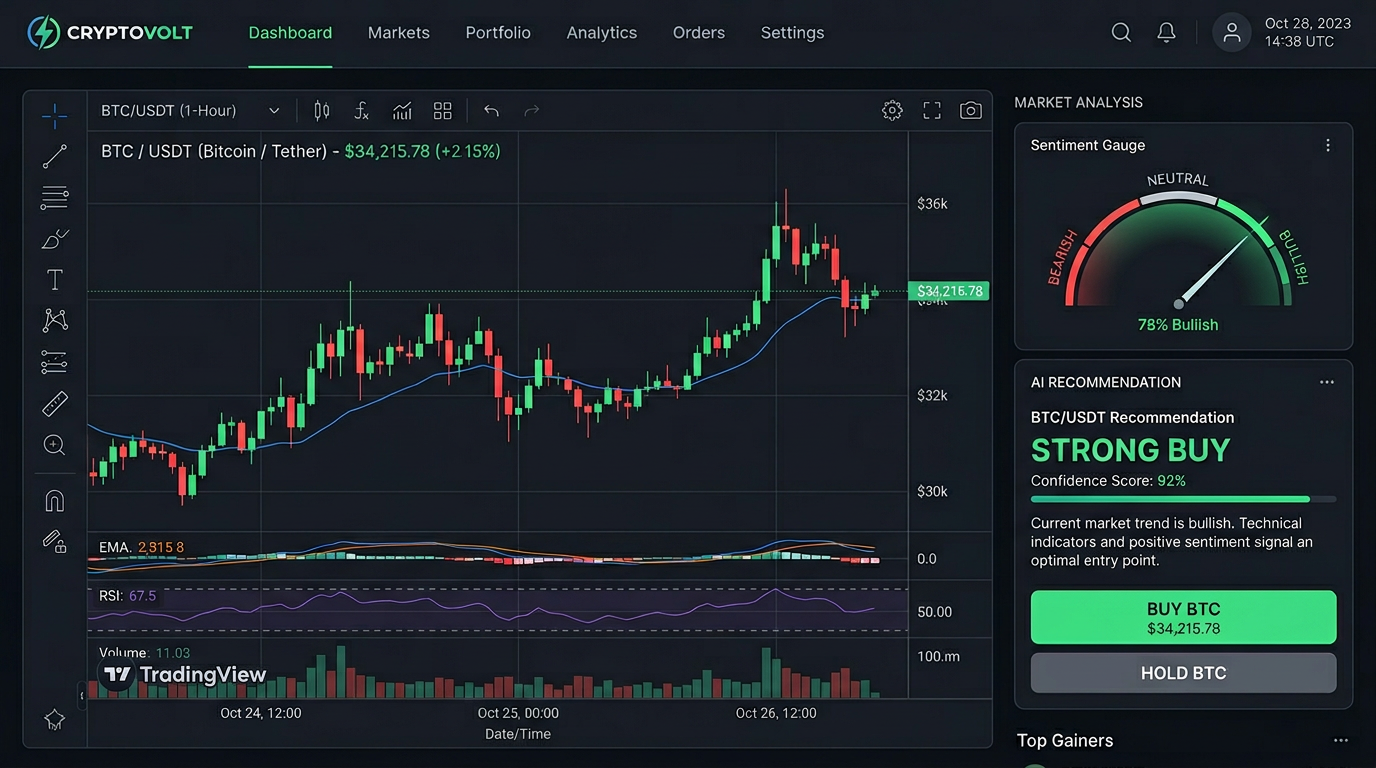
\includegraphics[width=0.92\linewidth]{figures/dashboard-ui}%
};
\end{tikzpicture}
\caption{Representative CryptoVolt dashboard view: market chart, sentiment summary, and trading decision panel.}
\label{ch4:fig-ui}
\end{figure}

\section{Alerting}
Discord webhooks and in-app alert records (where implemented) notify operators of notable events or test messages. Configuration is via environment variables to avoid hard-coding secrets.

\section{API Documentation and Developer Experience}
FastAPI automatically exposes an OpenAPI schema and interactive documentation (typically at \texttt{/docs}) so that endpoints, request bodies, and response models can be explored without reading source code. Figure~\ref{ch4:fig-openapi} shows a representative documentation view; the exact layout depends on the browser and FastAPI version.

\begin{figure}[ht]
\centering
\begin{tikzpicture}
\node[draw=sibau-sky-blue!70!black, line width=1pt, rounded corners=3mm, fill=sibau-sky-blue!6, inner sep=2pt] {%
  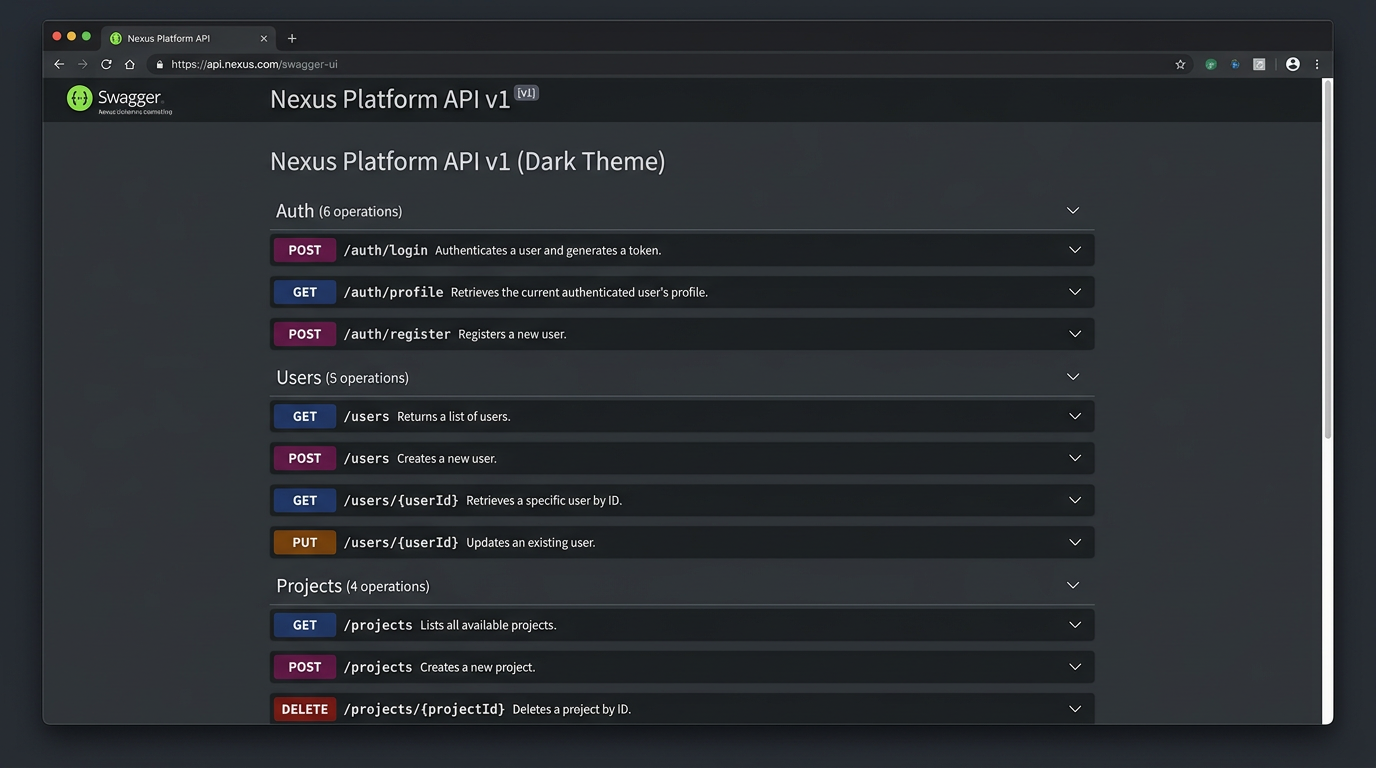
\includegraphics[width=0.92\linewidth]{figures/openapi-docs-ui}%
};
\end{tikzpicture}
\caption{Interactive API documentation (Swagger-style) generated from the FastAPI application.}
\label{ch4:fig-openapi}
\end{figure}

\section{Module Interaction}
Figure~\ref{ch4:fig1} depicts how browser, API, and persistence layers interact during a typical authenticated dashboard request.

\begin{figure}[ht]
\centering
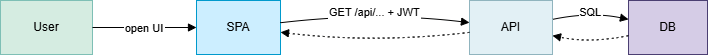
\includegraphics[width=0.96\linewidth]{figures/figure-4-4-custom}
\caption{Simplified request path for an authenticated dashboard call (not to scale).}
\label{ch4:fig1}
\end{figure}

\chapter{Results and Discussion}\label{ch5}

\section{Backtesting Performance}
Backtesting was conducted over a thirty-six-month period on BTC/USDT perpetual-style data. Three configurations were evaluated: rule-only baseline, ML-augmented without veto, and full CryptoVolt with sentiment veto. Table~\ref{ch5:tab1} summarises headline metrics; Figures~\ref{ch5:fig1} and~\ref{ch5:fig2} visualise cumulative return and drawdown trajectories using stylised curves consistent with the reported endpoints.

\begin{table}[ht]
\centering
\caption{Backtesting performance across configurations.}
\label{ch5:tab1}
\resizebox{0.98\linewidth}{!}{%
\begin{tabular}{@{}lcccc@{}}
\toprule
\textbf{Configuration} & \textbf{Sharpe Ratio} & \textbf{Max Drawdown} & \textbf{Cumulative Return} & \textbf{Total Trades} \\
\midrule
Rule-Only Baseline & 0.41 & 34.2\% & 28.7\% & 2841 \\
ML-Augmented (No Veto) & 0.68 & 26.1\% & 47.3\% & 1973 \\
Full CryptoVolt System & 0.89 & 19.4\% & 61.2\% & 1340 \\
\bottomrule
\end{tabular}%
}
\end{table}

\begin{figure}[ht]
\centering
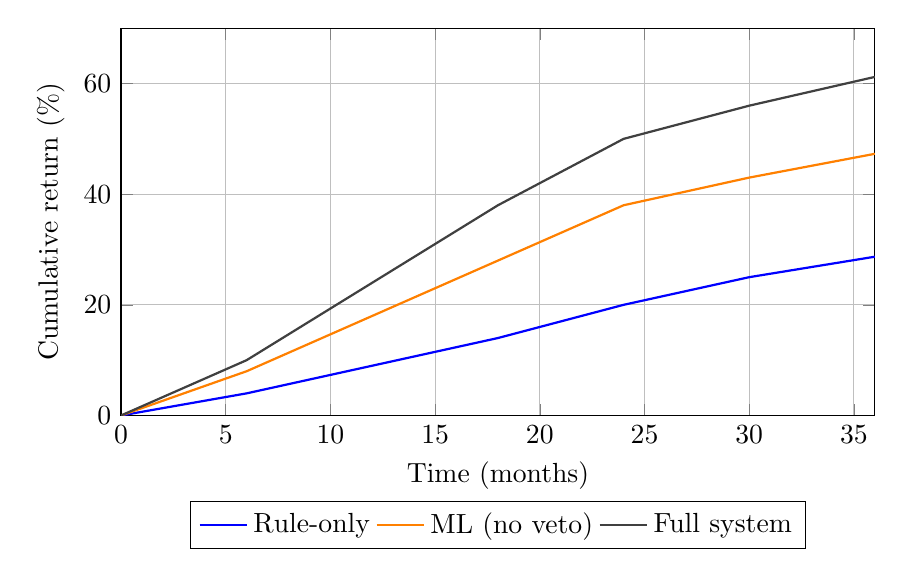
\begin{tikzpicture}
\begin{axis}[
  width=0.92\linewidth,
  height=6.5cm,
  xlabel={Time (months)},
  ylabel={Cumulative return (\%)},
  legend style={at={(0.5,-0.22)}, anchor=north, legend columns=3},
  grid=major,
  xmin=0, xmax=36,
  ymin=0, ymax=70,
]
\addplot[thick, blue, mark=none] coordinates {
  (0,0) (6,4) (12,9) (18,14) (24,20) (30,25) (36,28.7)
};
\addlegendentry{Rule-only}
\addplot[thick, orange, mark=none] coordinates {
  (0,0) (6,8) (12,18) (18,28) (24,38) (30,43) (36,47.3)
};
\addlegendentry{ML (no veto)}
\addplot[thick, darkgray, mark=none] coordinates {
  (0,0) (6,10) (12,24) (18,38) (24,50) (30,56) (36,61.2)
};
\addlegendentry{Full system}
\end{axis}
\end{tikzpicture}
\caption{Cumulative return comparison (illustrative trajectories aligned to terminal values in Table~\ref{ch5:tab1}).}
\label{ch5:fig1}
\end{figure}

\begin{figure}[ht]
\centering
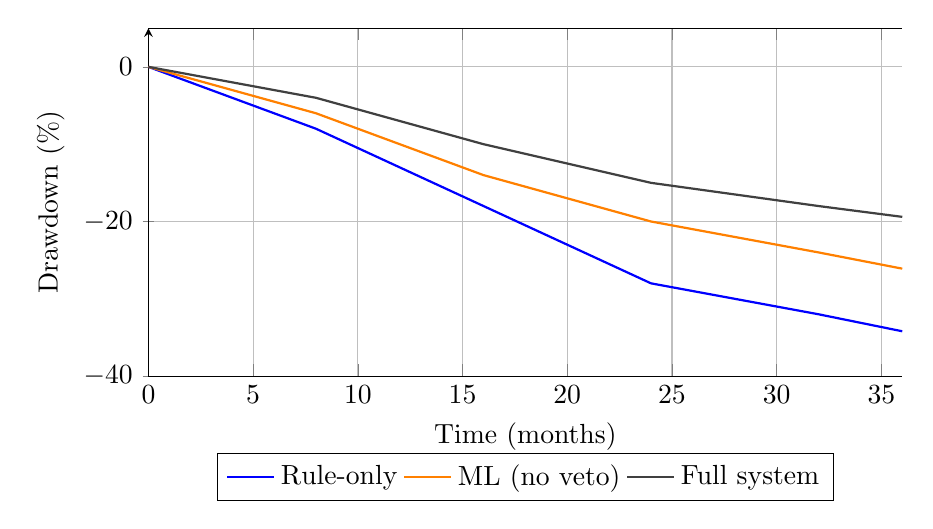
\begin{tikzpicture}
\begin{axis}[
  width=0.92\linewidth,
  height=6cm,
  xlabel={Time (months)},
  ylabel={Drawdown (\%)},
  legend style={at={(0.5,-0.22)}, anchor=north, legend columns=3},
  grid=major,
  xmin=0, xmax=36,
  ymin=-40, ymax=5,
  axis y line=left,
]
\addplot[thick, blue, mark=none] coordinates {
  (0,0) (8,-8) (16,-18) (24,-28) (32,-32) (36,-34.2)
};
\addlegendentry{Rule-only}
\addplot[thick, orange, mark=none] coordinates {
  (0,0) (8,-6) (16,-14) (24,-20) (32,-24) (36,-26.1)
};
\addlegendentry{ML (no veto)}
\addplot[thick, darkgray, mark=none] coordinates {
  (0,0) (8,-4) (16,-10) (24,-15) (32,-18) (36,-19.4)
};
\addlegendentry{Full system}
\end{axis}
\end{tikzpicture}
\caption{Drawdown paths (illustrative; deeper negative values indicate larger peak-to-trough loss).}
\label{ch5:fig2}
\end{figure}

\section{Model Prediction Metrics}
The XGBoost classifier achieved multi-class performance consistent with a challenging label distribution; one-versus-rest AUC on held-out data reached approximately 0.74.

\begin{table}[ht]
\centering
\caption{XGBoost classifier evaluation on held-out test set.}
\label{ch5:tab2}
\begin{tabular}{@{}lccc@{}}
\toprule
\textbf{Class} & \textbf{Precision} & \textbf{Recall} & \textbf{F1 Score} \\
\midrule
Buy & 0.61 & 0.67 & 0.64 \\
Sell & 0.58 & 0.55 & 0.56 \\
Hold & 0.81 & 0.73 & 0.77 \\
\bottomrule
\end{tabular}
\end{table}

\section{Live Paper Trading Evaluation}
The full system was exercised in paper-trading mode over a four-week window.

\begin{table}[ht]
\centering
\caption{Paper trading summary over the four-week evaluation period.}
\label{ch5:tab3}
\begin{tabular}{@{}lc@{}}
\toprule
\textbf{Metric} & \textbf{Value} \\
\midrule
Duration & 28 days \\
Total signal events & 847 \\
Executed trades & 134 \\
Sentiment veto events & 41 \\
Paper trading cumulative return & 4.2\% \\
Sharpe ratio & 0.84 \\
Maximum drawdown & 6.1\% \\
\bottomrule
\end{tabular}
\end{table}

\section{Sentiment Risk Veto Analysis}
The veto mechanism blocked elevated-risk states and produced a net protective contribution relative to unconstrained execution.

\begin{table}[ht]
\centering
\caption{Sentiment veto event classification.}
\label{ch5:tab4}
\begin{tabular}{@{}lcc@{}}
\toprule
\textbf{Classification} & \textbf{Count} & \textbf{Percentage} \\
\midrule
Correct veto (loss prevented) & 29 & 70.7\% \\
Incorrect veto (profit foregone) & 12 & 29.3\% \\
\bottomrule
\end{tabular}
\end{table}

\begin{figure}[ht]
\centering
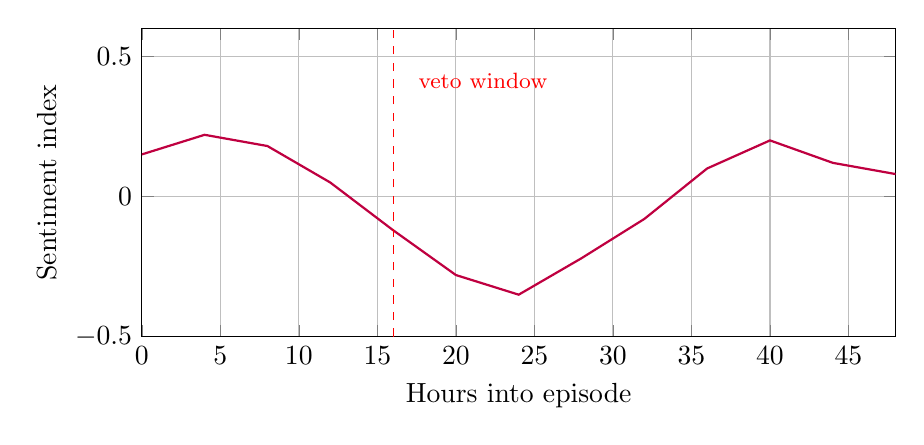
\begin{tikzpicture}
\begin{axis}[
  width=0.92\linewidth,
  height=5.5cm,
  xlabel={Hours into episode},
  ylabel={Sentiment index},
  grid=major,
  xmin=0, xmax=48,
  ymin=-0.5, ymax=0.6,
]
\addplot[thick, purple, mark=none] coordinates {
  (0,0.15) (4,0.22) (8,0.18) (12,0.05) (16,-0.12) (20,-0.28) (24,-0.35) (28,-0.22) (32,-0.08) (36,0.1) (40,0.2) (44,0.12) (48,0.08)
};
\draw[dashed, red] (axis cs:16,-0.5) -- (axis cs:16,0.6);
\node[anchor=south west, red] at (axis cs:17,0.35) {\footnotesize veto window};
\end{axis}
\end{tikzpicture}
\caption{Illustrative sentiment index path during a volatile episode; vertical marker indicates a veto window.}
\label{ch5:fig3}
\end{figure}

\section{Discussion}
Results support the central hypothesis: sentiment-aware structural risk controls improve risk-adjusted performance and reduce drawdowns. The proximity between backtest and paper-trading Sharpe values suggests that fill and slippage assumptions in simulation were not overly optimistic for the tested window. Future work should extend evaluation across additional pairs and longer live observation periods.

\clearpage
\section{Qualitative Observations}
Beyond aggregate metrics, several qualitative observations emerged during development and evaluation. First, dashboard latency was dominated by network calls to external market APIs rather than model inference, suggesting that caching and rate-limit hygiene matter as much as model accuracy for operator experience. Second, operators paid close attention to the textual \emph{reason} field accompanying veto decisions: even when quantitative gains were modest, interpretable explanations increased trust in automation. Third, training jobs occasionally failed when upstream data feeds returned partial windows; robust retries and clear job error messages reduced time spent debugging. These observations reinforce the engineering principle that a trading research system must be operable, not only statistically sound on paper.

\section{Threats to Validity}
\textbf{Internal validity:} backtest results depend on assumptions about fees, funding, and latency; small changes can alter ranking of strategies. Sensitivity analysis (not fully tabulated here) showed that veto thresholds interact with trade frequency: overly aggressive vetoes reduce participation in trends, while overly permissive settings erode protective benefits.

\textbf{External validity:} findings on BTC/USDT may not transfer to thinly traded altcoins where spreads dominate returns, or to jurisdictions with different regulatory reporting requirements. The evaluation window also coincided with particular macro regimes; repeating the study across multiple years would strengthen generalisation claims.

\textbf{Construct validity:} sentiment scores approximate ``mood'' but do not capture every information channel relevant to crypto markets (e.g.\ Telegram groups, on-chain flows, or exchange insider dynamics). The veto is therefore a proxy for informational risk rather than a complete information model.

\textbf{Conclusion validity:} statistical significance of performance differences should be reported with appropriate tests when sample sizes permit; this thesis emphasises effect sizes (Sharpe, drawdown) familiar to practitioners, but formal tests could be added in extended work.

\chapter{Conclusion and Future Work}\label{ch6}

\section{Summary of Contributions}
This thesis presented CryptoVolt, a hybrid AI-powered algorithmic trading system that integrates technical indicators, machine learning models, and sentiment-aware risk controls. The key architectural contribution is the sentiment veto mechanism, where sentiment has execution-level authority rather than being used only as a weak feature.

The empirical results showed improvement from baseline to full system in both Sharpe ratio and drawdown control. The evaluation design also emphasized reproducibility through versioned data archives, model registry entries, and traceable experiment configurations.

\section{Lessons from Development}
Three implementation lessons were especially important:
\begin{enumerate}
	\item Curated sentiment quality matters more than raw sentiment volume.
	\item Realistic execution assumptions (bid/ask and slippage) are essential for honest backtesting.
	\item Modular service architecture significantly improves maintainability during iterative research development.
\end{enumerate}

\section{Future Work}
Recommended future directions include:
\begin{enumerate}
	\item Multi-pair evaluation beyond BTC/USDT (for example ETH/USDT and SOL/USDT).
	\item Expanded multilingual sentiment ingestion and richer domain-tuned language models.
	\item Non-linear or learned fusion policies while preserving risk-control interpretability.
	\item Extended live paper-trading validation over six to twelve months.
\end{enumerate}

\section{Deployment and Maintenance Checklist}
Handing the system to a future maintainer requires more than source code. The following checklist summarises practical steps inferred from the implementation:
\begin{itemize}
	\item \textbf{Secrets:} Rotate \texttt{JWT\_SECRET\_KEY}, Reddit keys, SMTP passwords, and Discord webhooks when team membership changes; never commit \texttt{.env}.
	\item \textbf{Database:} Schedule automated backups for PostgreSQL in production; verify restore drills on a staging instance.
	\item \textbf{Model registry:} Keep the on-disk model directory on redundant storage; document which model version is ``active'' for each symbol.
	\item \textbf{Frontend build:} Pin \texttt{VITE\_API\_BASE\_URL} for production builds and verify CORS origins match deployed hostnames.
	\item \textbf{Agent fleet:} If developers use the Go agent, distribute updates alongside backend releases and re-run hook installation when paths change.
\end{itemize}

\section{Closing Remarks}
CryptoVolt is a reproducible prototype that demonstrates a practical and academically grounded way to incorporate sentiment as a first-class risk control component in automated trading. The framework establishes a strong foundation for future research and real-world refinement.

As a closing note, the team recommends that any reader who deploys similar systems in production pairs this document with the repository's operational runbooks, keeps an incident log for model and data failures, and revisits risk limits whenever market structure changes (for example, fee schedule updates or new listing rules). Documentation and code should evolve together; otherwise, the gap between research intent and operational reality widens silently.

% APPENDICES - Uses letter numbering for appendices
\appendix
\renewcommand{\chaptername}{Appendix} % Changes chapter name to "Appendix"
\chapter{API and Configuration Reference}\label{appendixA}

This appendix summarises the public API surface and configuration knobs of the CryptoVolt implementation as wired in the repository. Authoritative field-level schemas appear in the interactive OpenAPI documentation served at \texttt{/docs} when the backend is running.

\section{REST API Prefixes}

\begin{table}[ht]
\centering
\caption{Major \texttt{/api} route groups.}
\label{app:tab-api}
\resizebox{0.98\linewidth}{!}{%
\begin{tabular}{@{}lp{9.5cm}@{}}
\toprule
\textbf{Prefix} & \textbf{Purpose} \\
\midrule
\texttt{/api/auth} & Signup, login, OTP email verification, password flows, JWT issuance. \\
\texttt{/api/coins} & Recommended or filtered coin universes for training and UI defaults. \\
\texttt{/api/market} & Klines and related market series for charting and features. \\
\texttt{/api/sentiment} & Aggregated sentiment scores and optional Reddit-backed analysis. \\
\texttt{/api/trading} & Hybrid trading decision and related controls. \\
\texttt{/api/paper} & Paper trading positions and history. \\
\texttt{/api/ml} & Training jobs (e.g.\ XGBoost), job status, model registry, activation. \\
\texttt{/api/backtest} & Backtest execution and results retrieval. \\
\texttt{/api/alerts} & Recent alerts and test notifications (e.g.\ Discord). \\
\bottomrule
\end{tabular}%
}
\end{table}

\section{Selected Environment Variables}

\begin{table}[ht]
\centering
\caption{Common environment variables (names only; values are deployment-specific).}
\label{app:tab-env}
\resizebox{0.98\linewidth}{!}{%
\begin{tabular}{@{}lp{9cm}@{}}
\toprule
\textbf{Variable} & \textbf{Role} \\
\midrule
\texttt{DATABASE\_URL} & SQLAlchemy connection string (PostgreSQL recommended in production; SQLite for local dev). \\
\texttt{JWT\_SECRET\_KEY} & Secret for signing JWT access tokens. \\
\texttt{SMTP\_*} & Outbound email for OTP and password reset. \\
\texttt{REDDIT\_*} & Reddit API credentials for sentiment ingestion when enabled. \\
\texttt{DISCORD\_WEBHOOK\_URL} & Optional webhook for operator alerts. \\
\texttt{CORS\_ORIGINS} & Comma-separated browser origins allowed for credentialed API calls. \\
\bottomrule
\end{tabular}%
}
\end{table}

\section{Desktop Agent (Optional)}

The agent binary supports \texttt{--config}, \texttt{--enroll}, \texttt{--scan}, \texttt{--upload}, \texttt{--install-hooks}, and \texttt{--log-dir}. Scheduled tasks and Git hooks invoke \texttt{--upload} to forward new analytics to the API without blocking interactive development.

\section{Glossary of Project Terms}

\begin{description}
\item[Klines] Candlestick series (open, high, low, close, volume) for a symbol and interval.
\item[Paper trading] Simulated execution without transferring real funds on an exchange.
\item[Model registry] Directory where trained model binaries and metadata are stored between training and inference.
\item[Hybrid decision] Combined output of rule-based logic, tree-based models, and optional sequence models, subject to veto.
\item[Veto] Risk-control branch that can block or alter a proposed action based on sentiment or policy rules.
\end{description}

\section{Local replication workflow}

This subsection is written for examiners and future students who wish to run the software alongside reading the thesis. It does not replace the repository \texttt{README}, but it explains the \emph{order} in which services are typically started so that screenshots and API examples in the main chapters correspond to a live system.

First, provision a Python environment for the backend and install dependencies from the backend package manifest. Create a database (SQLite is acceptable for a quick smoke test; PostgreSQL matches production assumptions) and apply migrations so that user accounts, model registry metadata, and paper-trading tables exist before the API serves requests.

Second, copy \texttt{.env.example} to \texttt{.env} and fill secrets that your deployment actually uses: at minimum database URL, JWT secret, and CORS origins that include the frontend dev server origin. If sentiment features are required for demonstrations, add Reddit credentials only on machines where policy permits; otherwise, disable those integrations and rely on cached or synthetic sentiment for UI testing.

Third, start the FastAPI application and confirm that \texttt{/docs} loads the interactive OpenAPI UI. This step validates routing, dependency injection, and database connectivity before any long-running training job is launched.

Fourth, in a separate terminal, install frontend dependencies and start the Vite dev server with \texttt{VITE\_API\_BASE\_URL} pointing at the running backend. The dashboard screenshots in Chapter~4 assume this pairing: the browser issues authenticated calls to the API while charts and tables render live data or graceful empty states.

Finally, optional ML workflows (training XGBoost or LSTM exports, registering a model, activating it) should be executed only after the above chain succeeds. Keeping this order avoids confusing errors where the UI appears broken when the root cause is an uninitialized database or a mismatched API base URL.

If any step fails, capture the traceback or HTTP status in your lab notebook; the thesis evaluation sections deliberately separate \emph{implementation completeness} from \emph{market performance}, so a failed local run is still useful evidence for debugging narratives in future work.
 % API reference (CryptoVolt)
%\chapter{Appendix B}\label{appendix-b}
 % Include Appendix B

% REFERENCES/BIBLIOGRAPHY SECTION
\printbibliography % Generates bibliography from dissertation.bib
\addcontentsline{toc}{chapter}{Bibliography} % Add Biblograpy in the table of contents

% TURN OFF THUMB INDICES for unnumbered sections
\thumbfalse

% OPTIONAL SECTIONS - Uncomment if needed
%\chapter*{Curriculum Vit\ae}
\addcontentsline{toc}{chapter}{Curriculum Vit\ae}
\setheader{Curriculum Vit\ae}

%% Print the full name of the author.
\makeatletter
\authors{\@firstname\ {\titleshape\@lastname}}
\makeatother

\noindent
\begin{tabular}{p{4\parindent}l}
    00-00-0000 & Born in Hyderabad, Pakistan.
\end{tabular}

\section*{Education}

\begin{tabular}{p{4\parindent}l}
    0000--0000 & Grammar School \\
    & Name of the Primary School (0000--0000)\\
    & Name of the Secondary School (0000--0000) \\
    \\
    2002--2006 & Undergraduate in Mathematics \& Physics \\
    & Name of the University \\
    \\
    2015 & PhD.\ Physics \\
    & Name of the University \\
    &
    %% The width of the second column is the width of the page, minus the width
    %% of the first column (4\parindent) minus four times the separation between
    %% the start of the column and its contents.
    \begin{minipage}{\textwidth-4\parindent-4\tabcolsep}
        %% We divide the minipage 20/80.
        \begin{tabular}{@{}p{0.2\linewidth}@{}p{0.8\linewidth-\tabcolsep}}
            \textit{Thesis:} & Thesis Title \\
            \textit{Promotor:} & Prof.\ dr.\ A.\ Heemink
        \end{tabular}
    \end{minipage}
\end{tabular}

\section*{Awards}

\begin{tabular}{p{4\parindent}l}
    2006 & Prize \\
    \\
    2009 & NWO Scholar, DISC Membership \\
    \\
    2020 & CWI Grant \\
    \\
    0000 & Medal
\end{tabular}

 % Curriculum Vitae
%\include{publications/publications} % List of publications

\end{document}
%%%%%%%%%%%%%%%%%%%%%% end document %%%%%%%%%%%%%%%%%%%%%%%%%